% Options for packages loaded elsewhere
% Options for packages loaded elsewhere
\PassOptionsToPackage{unicode}{hyperref}
\PassOptionsToPackage{hyphens}{url}
\PassOptionsToPackage{dvipsnames,svgnames,x11names}{xcolor}
%
\documentclass[
  11pt,
  a4paper,
]{article}
\usepackage{xcolor}
\usepackage[margin=2.5cm]{geometry}
\usepackage{amsmath,amssymb}
\setcounter{secnumdepth}{5}
\usepackage{iftex}
\ifPDFTeX
  \usepackage[T1]{fontenc}
  \usepackage[utf8]{inputenc}
  \usepackage{textcomp} % provide euro and other symbols
\else % if luatex or xetex
  \usepackage{unicode-math} % this also loads fontspec
  \defaultfontfeatures{Scale=MatchLowercase}
  \defaultfontfeatures[\rmfamily]{Ligatures=TeX,Scale=1}
\fi
\usepackage{lmodern}
\ifPDFTeX\else
  % xetex/luatex font selection
\fi
% Use upquote if available, for straight quotes in verbatim environments
\IfFileExists{upquote.sty}{\usepackage{upquote}}{}
\IfFileExists{microtype.sty}{% use microtype if available
  \usepackage[]{microtype}
  \UseMicrotypeSet[protrusion]{basicmath} % disable protrusion for tt fonts
}{}
\makeatletter
\@ifundefined{KOMAClassName}{% if non-KOMA class
  \IfFileExists{parskip.sty}{%
    \usepackage{parskip}
  }{% else
    \setlength{\parindent}{0pt}
    \setlength{\parskip}{6pt plus 2pt minus 1pt}}
}{% if KOMA class
  \KOMAoptions{parskip=half}}
\makeatother
% Make \paragraph and \subparagraph free-standing
\makeatletter
\ifx\paragraph\undefined\else
  \let\oldparagraph\paragraph
  \renewcommand{\paragraph}{
    \@ifstar
      \xxxParagraphStar
      \xxxParagraphNoStar
  }
  \newcommand{\xxxParagraphStar}[1]{\oldparagraph*{#1}\mbox{}}
  \newcommand{\xxxParagraphNoStar}[1]{\oldparagraph{#1}\mbox{}}
\fi
\ifx\subparagraph\undefined\else
  \let\oldsubparagraph\subparagraph
  \renewcommand{\subparagraph}{
    \@ifstar
      \xxxSubParagraphStar
      \xxxSubParagraphNoStar
  }
  \newcommand{\xxxSubParagraphStar}[1]{\oldsubparagraph*{#1}\mbox{}}
  \newcommand{\xxxSubParagraphNoStar}[1]{\oldsubparagraph{#1}\mbox{}}
\fi
\makeatother


\usepackage{longtable,booktabs,array}
\newcounter{none} % for unnumbered tables
\usepackage{calc} % for calculating minipage widths
% Correct order of tables after \paragraph or \subparagraph
\usepackage{etoolbox}
\makeatletter
\patchcmd\longtable{\par}{\if@noskipsec\mbox{}\fi\par}{}{}
\makeatother
% Allow footnotes in longtable head/foot
\IfFileExists{footnotehyper.sty}{\usepackage{footnotehyper}}{\usepackage{footnote}}
\makesavenoteenv{longtable}
\usepackage{graphicx}
\makeatletter
\newsavebox\pandoc@box
\newcommand*\pandocbounded[1]{% scales image to fit in text height/width
  \sbox\pandoc@box{#1}%
  \Gscale@div\@tempa{\textheight}{\dimexpr\ht\pandoc@box+\dp\pandoc@box\relax}%
  \Gscale@div\@tempb{\linewidth}{\wd\pandoc@box}%
  \ifdim\@tempb\p@<\@tempa\p@\let\@tempa\@tempb\fi% select the smaller of both
  \ifdim\@tempa\p@<\p@\scalebox{\@tempa}{\usebox\pandoc@box}%
  \else\usebox{\pandoc@box}%
  \fi%
}
% Set default figure placement to htbp
\def\fps@figure{htbp}
\makeatother





\setlength{\emergencystretch}{3em} % prevent overfull lines

\providecommand{\tightlist}{%
  \setlength{\itemsep}{0pt}\setlength{\parskip}{0pt}}



 


\usepackage{booktabs}
\usepackage{longtable}
\usepackage{array}
\usepackage{multirow}
\usepackage{wrapfig}
\usepackage{float}
\usepackage{colortbl}
\usepackage{pdflscape}
\usepackage{tabu}
\usepackage{threeparttable}
\usepackage{threeparttablex}
\usepackage[normalem]{ulem}
\usepackage{makecell}
\usepackage{xcolor}
\usepackage{amsmath,amssymb,amsfonts}
\usepackage{graphicx}
\usepackage{booktabs}
\usepackage{longtable}
\usepackage{float}
\usepackage{fancyhdr}
\pagestyle{fancy}
\fancyhf{}
\fancyhead[L]{\small Why Have House Prices in Turkey Gone Up?}
\fancyhead[R]{\small EMU660 -- Hacettepe University}
\fancyfoot[C]{\thepage}
\setlength{\parindent}{4mm}
\usepackage[font=footnotesize,labelfont=bf]{caption}
\makeatletter
\@ifpackageloaded{caption}{}{\usepackage{caption}}
\AtBeginDocument{%
\ifdefined\contentsname
  \renewcommand*\contentsname{Table of contents}
\else
  \newcommand\contentsname{Table of contents}
\fi
\ifdefined\listfigurename
  \renewcommand*\listfigurename{List of Figures}
\else
  \newcommand\listfigurename{List of Figures}
\fi
\ifdefined\listtablename
  \renewcommand*\listtablename{List of Tables}
\else
  \newcommand\listtablename{List of Tables}
\fi
\ifdefined\figurename
  \renewcommand*\figurename{Figure}
\else
  \newcommand\figurename{Figure}
\fi
\ifdefined\tablename
  \renewcommand*\tablename{Table}
\else
  \newcommand\tablename{Table}
\fi
}
\@ifpackageloaded{float}{}{\usepackage{float}}
\floatstyle{ruled}
\@ifundefined{c@chapter}{\newfloat{codelisting}{h}{lop}}{\newfloat{codelisting}{h}{lop}[chapter]}
\floatname{codelisting}{Listing}
\newcommand*\listoflistings{\listof{codelisting}{List of Listings}}
\makeatother
\makeatletter
\makeatother
\makeatletter
\@ifpackageloaded{caption}{}{\usepackage{caption}}
\@ifpackageloaded{subcaption}{}{\usepackage{subcaption}}
\makeatother
\usepackage{bookmark}
\IfFileExists{xurl.sty}{\usepackage{xurl}}{} % add URL line breaks if available
\urlstyle{same}
\hypersetup{
  pdftitle={Why Have House Prices in Turkey Gone Up in the Last Ten Years?},
  pdfauthor={Ömer Furkan Demirci; Fatih Alper Vural},
  colorlinks=true,
  linkcolor={blue},
  filecolor={Maroon},
  citecolor={Blue},
  urlcolor={blue},
  pdfcreator={LaTeX via pandoc}}


\title{Why Have House Prices in Turkey Gone Up in the Last Ten Years?}
\usepackage{etoolbox}
\makeatletter
\providecommand{\subtitle}[1]{% add subtitle to \maketitle
  \apptocmd{\@title}{\par {\large #1 \par}}{}{}
}
\makeatother
\subtitle{Project Final Report\\
EMU660 Statistical Learning and Analytics}
\author{Ömer Furkan Demirci \and Fatih Alper Vural}
\date{May 18, 2026}
\begin{document}
\maketitle

\renewcommand*\contentsname{Table of contents}
{
\setcounter{tocdepth}{3}
\tableofcontents
}

\newpage

\subsection*{Abstract}\label{abstract}
\addcontentsline{toc}{subsection}{Abstract}

Housing affordability has emerged as one of the most pressing
socioeconomic challenges in Türkiye over the past decade. This study
investigates the key drivers of the sharp and sustained rise in housing
prices between 2014 and 2024, drawing on four official monthly
time-series datasets obtained from the Central Bank of the Republic of
Türkiye (TCMB/EVDS): the House Price Index (HPI), housing sales
statistics, USD/EUR exchange rates, and credit card sectoral expenditure
data. Through exploratory analysis, correlation testing, regional
comparison, and multiple linear regression modelling, we find that
exchange rate depreciation and broad consumer spending inflation are the
dominant macroeconomic forces behind rising house prices, while sales
volumes display an inverse relationship with price levels --- consistent
with demand compression at high price levels. Regional heterogeneity is
substantial: western coastal regions lead price growth, whereas interior
Anatolian regions lag considerably. Our model explains approximately
95--99\% of the variance in the national HPI, suggesting that
macroeconomic indicators are strong predictors of housing price
trajectories in Türkiye.

\begin{center}\rule{0.5\linewidth}{0.5pt}\end{center}

\newpage

\section{Introduction}\label{introduction}

Housing has become one of the most consequential economic and social
issues in Türkiye over the past ten years. After a period of moderate
growth, the national House Price Index (HPI) accelerated dramatically
beginning around 2019--2020, ultimately reaching levels that have placed
homeownership out of reach for large segments of the population.
Understanding the structural and macroeconomic causes of this surge is
essential for both policy design and economic analysis.

This report addresses the following research question:

\begin{quote}
\textbf{Why have house prices in Turkey gone up in the last ten years?}
\end{quote}

To answer this question we combine four monthly time-series datasets
from the Electronic Data Delivery System (EVDS) of the Central Bank of
the Republic of Türkiye (TCMB): the national and regional House Price
Index, housing sales statistics, USD/TRY and EUR/TRY exchange rates, and
credit card sectoral expenditure data. Our analytical approach proceeds
from descriptive exploration through correlation analysis and regional
comparison to multiple regression modelling, allowing us to quantify the
relative contributions of macroeconomic indicators.

The remainder of this report is organised as follows.
Section~\ref{sec-data} describes the datasets and preprocessing steps.
Section~\ref{sec-analysis} presents the full analysis, including trend
visualisation, correlation testing, regional comparison, and regression
modelling. Section~\ref{sec-results} summarises the key takeaways and
discusses limitations. A references section follows.

\section{Data}\label{sec-data}

\subsection{Data Source}\label{data-source}

All data were obtained from the \textbf{Electronic Data Delivery System
(EVDS)} of the Central Bank of the Republic of Türkiye (TCMB). EVDS
provides official, high-frequency economic data and is widely used for
academic and professional analysis.

The project draws on four datasets:

\begin{itemize}
\tightlist
\item
  \textbf{House Price Index (HPI)} --- monthly housing price index at
  national and regional (NUTS2) levels.
\item
  \textbf{House Sales Statistics} --- monthly housing sales data at the
  provincial level.
\item
  \textbf{Exchange Rates (USD/TRY, EUR/TRY)} --- monthly exchange rate
  series.
\item
  \textbf{Credit Card Sectoral Expenditures} --- monthly sector-based
  credit card spending data.
\end{itemize}

\subsection{General Information About the
Data}\label{general-information-about-the-data}

The processed dataset consists of three main analytical tables described
below.

\subsubsection{Exchange Rate Table}\label{exchange-rate-table}

This table contains Year, Month, USD/TRY conversion rate, and EUR/TRY
conversion rate columns. It represents monthly exchange rate movements
used as indicators of macroeconomic conditions and cost-side pressures.
Both series exhibit a strong upward trend over the sample period
(2014--2025), with the most dramatic depreciation occurring after 2021.

\subsubsection{Credit Card Expenditure
Table}\label{credit-card-expenditure-table}

This table contains Year, Month, Expense Type, and Quantity (spending
volume in millions of TRY). Sectoral credit card spending is used as a
broad nominal consumption proxy. As shown in
Table~\ref{tbl-top-categories}, the largest categories by cumulative
volume are e-commerce, supermarkets, food, clothing, and fuel.

\subsubsection{Housing Panel Dataset}\label{housing-panel-dataset}

This is the main analytical table. It contains Year, Month, Region
(NUTS2 level), House Price Index, and Total Sales (monthly units sold)
for each region. The national aggregate for Türkiye is included as a
separate row and is the primary object of the regression analysis.

\subsection{Preprocessing}\label{preprocessing}

The raw EVDS datasets were provided in Excel format and contained
heterogeneous structures (wide vs.~long) and different aggregation
levels (province vs.~region). Preprocessing was performed in Python
using \texttt{pandas} to standardise date formats, reshape wide datasets
to long format, translate coded column names (e.g., \texttt{KT2},
\texttt{TR62}) into meaningful labels, and aggregate province-level
sales data to NUTS2 regions consistent with the HPI structure.

\emph{Note: portions of the Python preprocessing code were developed
with assistance from AI language model tools. All analytical R code,
narrative interpretation, and conclusions are the authors' own work.}

\subsection{Potential Analyses}\label{potential-analyses}

Given the dataset characteristics, the following analytical directions
were pursued:

\begin{itemize}
\tightlist
\item
  Time-series trend visualisation of the HPI, exchange rates, and sales.
\item
  Year-over-year growth rate comparison.
\item
  Pearson correlation analysis between the HPI and macroeconomic
  covariates.
\item
  Regional comparison of HPI growth trajectories.
\item
  Multiple log-log regression modelling of HPI on exchange rates, sales,
  and credit card expenditure.
\end{itemize}

\section{Analysis}\label{sec-analysis}

\subsection{Exploratory Data Analysis}\label{exploratory-data-analysis}

We begin with descriptive statistics to understand the scale and
distribution of each key variable before examining relationships.

\begingroup\fontsize{9}{11}\selectfont

\begin{longtable}[t]{llllll}

\caption{\label{tbl-summary-stats}Summary statistics of key variables.}

\tabularnewline

\toprule
Variable & Min & Mean & Median & Max & SD\\
\midrule
\cellcolor{gray!10}{House Price Index} & \cellcolor{gray!10}{7.7} & \cellcolor{gray!10}{51.1} & \cellcolor{gray!10}{14.6} & \cellcolor{gray!10}{204.4} & \cellcolor{gray!10}{60.8}\\
Monthly Sales (units) & 45,218.0 & 126,140.7 & 120,437.5 & 265,223.0 & 35,718.6\\
\cellcolor{gray!10}{USD/TRY Rate} & \cellcolor{gray!10}{2.1} & \cellcolor{gray!10}{12.6} & \cellcolor{gray!10}{6.1} & \cellcolor{gray!10}{42.7} & \cellcolor{gray!10}{12.4}\\
EUR/TRY Rate & 2.7 & 13.9 & 6.8 & 49.9 & 13.7\\
\bottomrule

\end{longtable}

\endgroup{}

The HPI rose from a starting value near 7--8 to over 200 by the end of
the sample, reflecting the scale of the nominal price surge. Exchange
rates followed a similar upward trajectory, while monthly sales remained
considerably more volatile, suggesting that transaction volume decoupled
from price levels over time.

\begingroup\fontsize{9}{11}\selectfont

\begin{longtable}[t]{ll}

\caption{\label{tbl-top-categories}Top 8 credit card expenditure
categories --- cumulative total (2014--2025).}

\tabularnewline

\toprule
Expense Category & Total Spending (Billion TRY)\\
\midrule
\cellcolor{gray!10}{E-Alışveriş} & \cellcolor{gray!10}{15,913,640}\\
Market ve Alışveriş Merkezleri & 10,409,810\\
\cellcolor{gray!10}{Çeşitli Gıda} & \cellcolor{gray!10}{3,892,815}\\
Giyim ve Aksesuar & 3,889,505\\
\cellcolor{gray!10}{Benzin ve Yakıt İstasyonları} & \cellcolor{gray!10}{3,542,543}\\
\addlinespace
Hizmet Sektörleri & 3,486,972\\
\cellcolor{gray!10}{Elektrik-Elektronik Eşya / Bilgisayar} & \cellcolor{gray!10}{3,308,526}\\
Yemek & 3,156,894\\
\bottomrule

\end{longtable}

\endgroup{}

Credit card expenditure is dominated by e-commerce, retail, food, and
fuel. Total spending is used in this project as a broad proxy for the
nominal inflation environment rather than as a direct measure of housing
demand.

\subsection{Trend Analysis}\label{trend-analysis}

\subsubsection{House Price Index Over
Time}\label{house-price-index-over-time}

\begin{figure}[H]

\centering{

\pandocbounded{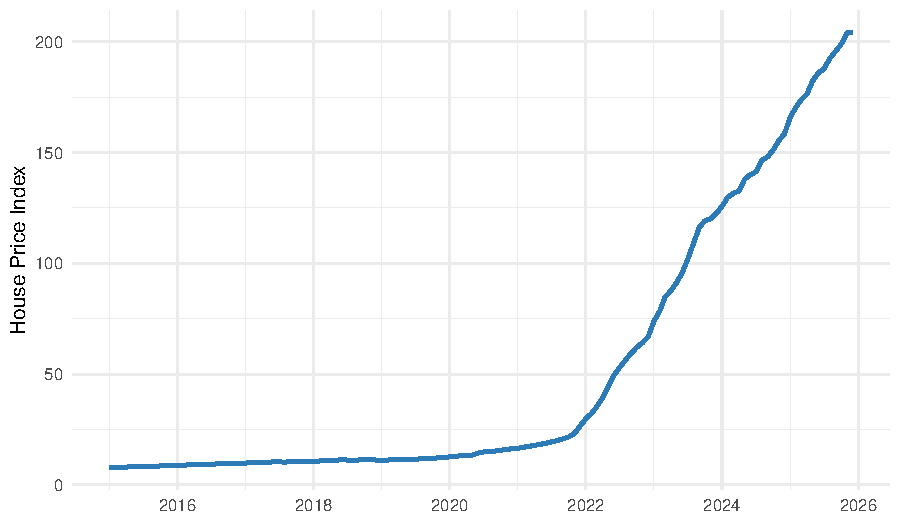
\includegraphics[keepaspectratio]{FAVURAL_EMU660_MiniPaper_files/figure-pdf/fig-hpi-trend-1.pdf}}

}

\caption{\label{fig-hpi-trend}National House Price Index over time
(2014--2025).}

\end{figure}%

The HPI remained relatively stable until 2019, then rose sharply
(Figure~\ref{fig-hpi-trend}). The steepest acceleration occurred during
2021--2023, coinciding with severe exchange rate depreciation and
historically high inflation rates in Türkiye. This timing is consistent
with a cost-push interpretation in which imported construction
materials, inflation expectations, and lira depreciation all contributed
to higher nominal house prices.

\subsubsection{Year-over-Year Growth Rate
Comparison}\label{year-over-year-growth-rate-comparison}

Raw index levels can make any two upward-trending series appear
correlated. Year-over-year (YoY) growth rates provide a more meaningful
diagnostic: they reveal whether sudden currency shocks coincide with
sudden house-price jumps.

\begin{figure}[H]

\centering{

\pandocbounded{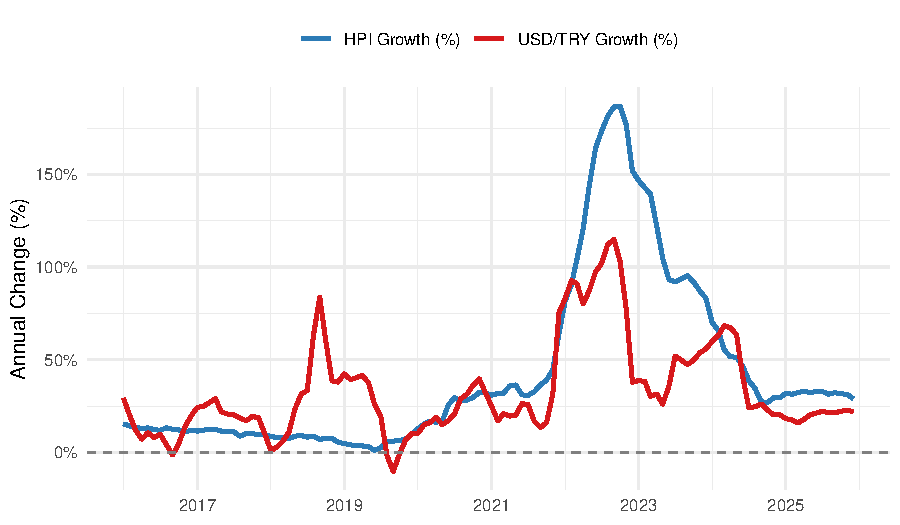
\includegraphics[keepaspectratio]{FAVURAL_EMU660_MiniPaper_files/figure-pdf/fig-yoy-1.pdf}}

}

\caption{\label{fig-yoy}Year-over-year growth rates: House Price Index
vs.~USD/TRY.}

\end{figure}%

As shown in Figure~\ref{fig-yoy}, major jumps in USD/TRY growth and HPI
growth occur in similar periods, especially the post-2020 acceleration.
This supports the view that exchange rate shocks and housing price
inflation are closely connected, though the chart documents co-movement
rather than a controlled causal estimate.

\subsubsection{Exchange Rates Over Time}\label{exchange-rates-over-time}

\begin{figure}[H]

\centering{

\pandocbounded{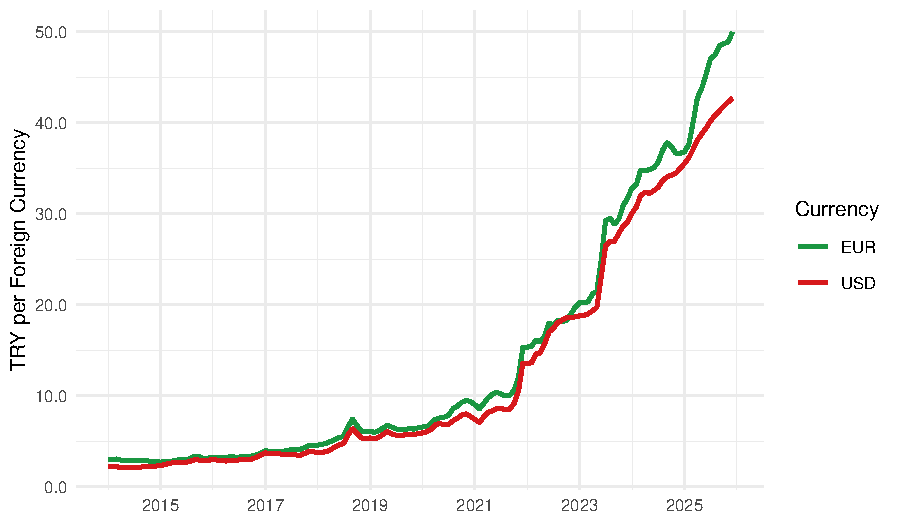
\includegraphics[keepaspectratio]{FAVURAL_EMU660_MiniPaper_files/figure-pdf/fig-fx-1.pdf}}

}

\caption{\label{fig-fx}USD/TRY and EUR/TRY exchange rates over the
sample period.}

\end{figure}%

\subsubsection{Annual Housing Sales}\label{annual-housing-sales}

\begin{figure}[H]

\centering{

\pandocbounded{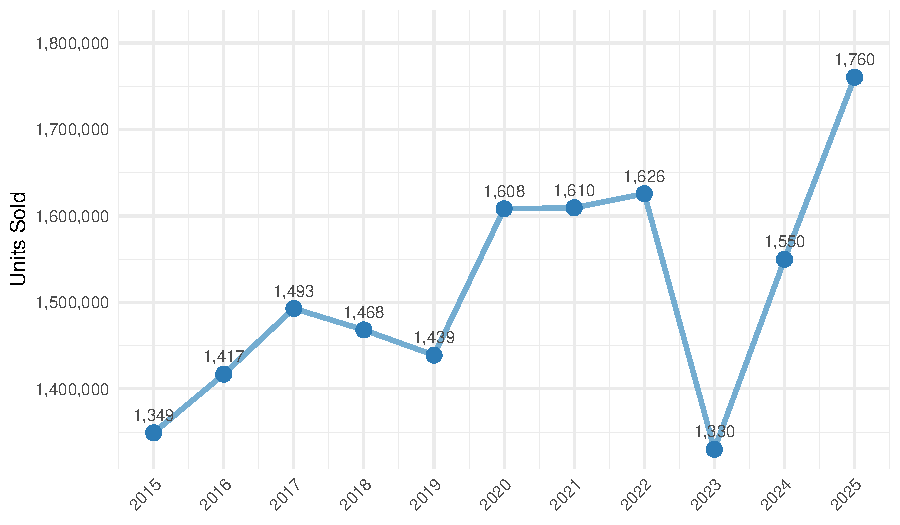
\includegraphics[keepaspectratio]{FAVURAL_EMU660_MiniPaper_files/figure-pdf/fig-sales-1.pdf}}

}

\caption{\label{fig-sales}Annual housing sales for Türkiye. Labels show
thousands of units sold.}

\end{figure}%

Sales fluctuated considerably over the sample period
(Figure~\ref{fig-sales}) with notable spikes in years of policy-driven
demand stimulus, but they did not sustain the same upward trend as the
HPI --- a first indication that price growth was not primarily
demand-driven.

\subsection{Correlation Analysis}\label{correlation-analysis}

\subsubsection{Correlation Heatmap}\label{correlation-heatmap}

A correlation heatmap summarises the pairwise relationships between all
key variables in a single, compact display.

\begin{figure}[H]

\centering{

\pandocbounded{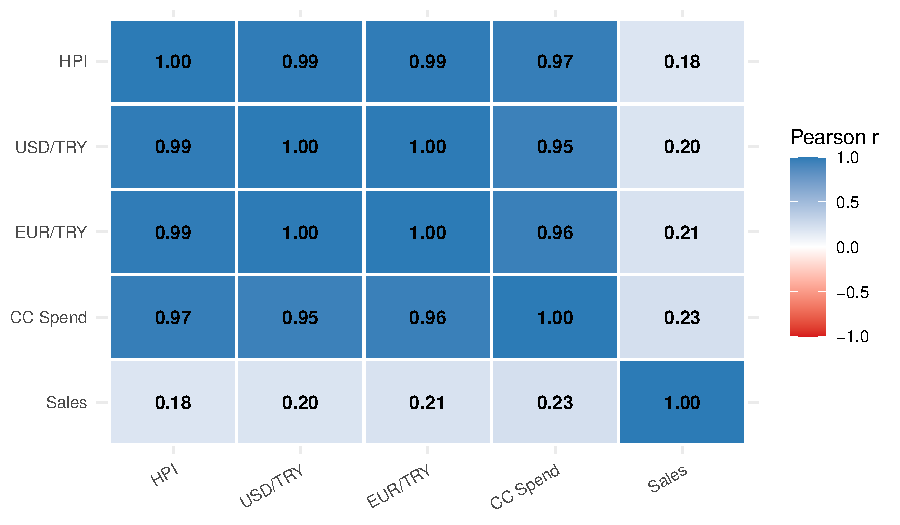
\includegraphics[keepaspectratio]{FAVURAL_EMU660_MiniPaper_files/figure-pdf/fig-corr-heatmap-1.pdf}}

}

\caption{\label{fig-corr-heatmap}Pearson correlation heatmap of key
variables.}

\end{figure}%

\begingroup\fontsize{9}{11}\selectfont

\begin{longtable}[t]{lr}

\caption{\label{tbl-corr}Pearson correlations with the House Price
Index.}

\tabularnewline

\toprule
Variable Pair & Pearson r\\
\midrule
\cellcolor{gray!10}{HPI vs USD/TRY} & \cellcolor{gray!10}{0.990}\\
HPI vs EUR/TRY & 0.990\\
\cellcolor{gray!10}{HPI vs CC Spend} & \cellcolor{gray!10}{0.973}\\
HPI vs Sales & 0.184\\
\bottomrule

\end{longtable}

\endgroup{}

The HPI exhibits very strong positive correlations with exchange rates
(\(r \approx 0.99\)) and credit card expenditure (\(r \approx 0.97\)),
but only a weak relationship with sales volume (\(r \approx 0.18\),
Table~\ref{tbl-corr}). Because all nominal variables trend upward over
time, these correlations may partly reflect shared non-stationarity; the
regression models and YoY analysis address this concern.

\subsubsection{Scatter Plot: log(HPI)
vs.~log(USD/TRY)}\label{scatter-plot-loghpi-vs.-logusdtry}

\begin{figure}[H]

\centering{

\pandocbounded{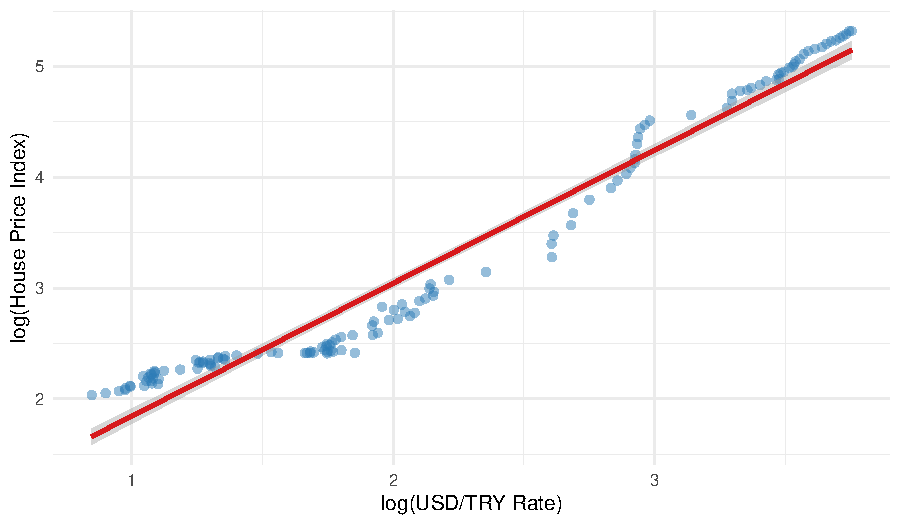
\includegraphics[keepaspectratio]{FAVURAL_EMU660_MiniPaper_files/figure-pdf/fig-scatter-1.pdf}}

}

\caption{\label{fig-scatter}Scatter plot of log(HPI) against
log(USD/TRY). Each point is one monthly observation.}

\end{figure}%

The scatter plot on log-transformed variables (Figure~\ref{fig-scatter})
shows a tight linear relationship with very little scatter, confirming
that the strong correlation is not merely an artefact of shared time
trends but persists across all levels of the exchange rate.

\subsection{Regional Comparison}\label{regional-comparison}

\subsubsection{Regional HPI
Trajectories}\label{regional-hpi-trajectories}

\begin{figure}[H]

\centering{

\pandocbounded{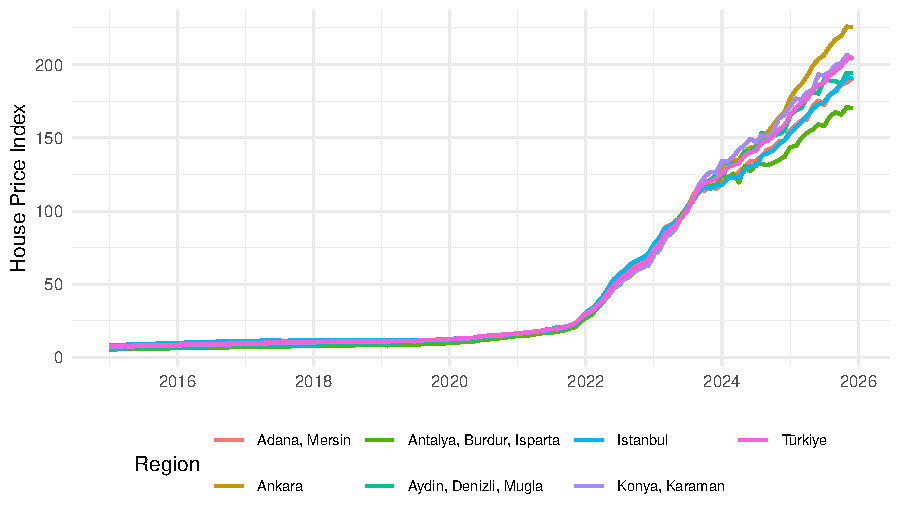
\includegraphics[keepaspectratio]{FAVURAL_EMU660_MiniPaper_files/figure-pdf/fig-regional-hpi-1.pdf}}

}

\caption{\label{fig-regional-hpi}House Price Index trajectories for
selected regions (2014--2025).}

\end{figure}%

\subsubsection{Regional Growth Ranking}\label{regional-growth-ranking}

\begin{figure}[H]

\centering{

\pandocbounded{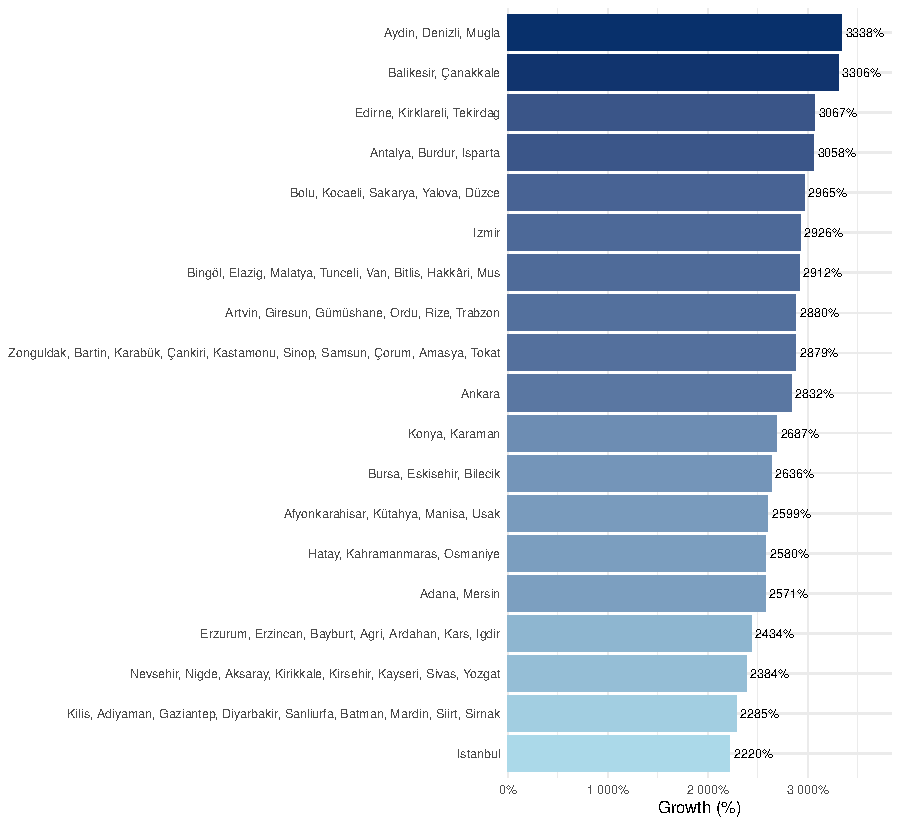
\includegraphics[keepaspectratio]{FAVURAL_EMU660_MiniPaper_files/figure-pdf/fig-regional-bar-1.pdf}}

}

\caption{\label{fig-regional-bar}Total HPI percentage growth by NUTS2
region (first to latest observation).}

\end{figure}%

\begin{table}

\caption{\label{tbl-regional-growth}HPI growth by NUTS2 region (first to
latest observation).}

\centering{

\begingroup\fontsize{8}{10}\selectfont

\begin{longtabu} to \linewidth {>{\raggedright}X>{\raggedright}X>{\raggedright}X>{\raggedleft}X}
\toprule
Region & First HPI & Latest HPI & Growth (\%)\\
\midrule
\cellcolor{gray!10}{Aydın, Denizli, Muğla} & \cellcolor{gray!10}{5.7} & \cellcolor{gray!10}{194.2} & \cellcolor{gray!10}{3337.5}\\
Balıkesir, Çanakkale & 6.2 & 211.9 & 3306.1\\
\cellcolor{gray!10}{Edirne, Kırklareli, Tekirdağ} & \cellcolor{gray!10}{6.2} & \cellcolor{gray!10}{196.1} & \cellcolor{gray!10}{3067.2}\\
Antalya, Burdur, Isparta & 5.4 & 170.2 & 3057.5\\
\cellcolor{gray!10}{Bolu, Kocaeli, Sakarya, Yalova, Düzce} & \cellcolor{gray!10}{6.9} & \cellcolor{gray!10}{210.9} & \cellcolor{gray!10}{2964.8}\\
\addlinespace
İzmir & 6.6 & 198.8 & 2926.5\\
\cellcolor{gray!10}{Bingöl, Elazığ, Malatya, Tunceli, Van, Bitlis, Hakkâri, Muş} & \cellcolor{gray!10}{8.2} & \cellcolor{gray!10}{245.8} & \cellcolor{gray!10}{2912.4}\\
Artvin, Giresun, Gümüşhane, Ordu, Rize, Trabzon & 7.4 & 219.7 & 2880.3\\
\cellcolor{gray!10}{Zonguldak, Bartın, Karabük, Çankırı, Kastamonu, Sinop, Samsun, Çorum, Amasya, Tokat} & \cellcolor{gray!10}{7.3} & \cellcolor{gray!10}{217.8} & \cellcolor{gray!10}{2879.1}\\
Ankara & 7.7 & 225.5 & 2831.9\\
\addlinespace
\cellcolor{gray!10}{Konya, Karaman} & \cellcolor{gray!10}{7.3} & \cellcolor{gray!10}{203.8} & \cellcolor{gray!10}{2687.3}\\
Bursa, Eskişehir, Bilecik & 7.4 & 203.0 & 2636.4\\
\cellcolor{gray!10}{Afyonkarahisar, Kütahya, Manisa, Uşak} & \cellcolor{gray!10}{8.5} & \cellcolor{gray!10}{228.9} & \cellcolor{gray!10}{2599.2}\\
Hatay, Kahramanmaraş, Osmaniye & 8.1 & 216.3 & 2580.2\\
\cellcolor{gray!10}{Adana, Mersin} & \cellcolor{gray!10}{7.1} & \cellcolor{gray!10}{190.7} & \cellcolor{gray!10}{2571.4}\\
\addlinespace
Türkiye & 7.7 & 204.4 & 2571.4\\
\cellcolor{gray!10}{Erzurum, Erzincan, Bayburt, Ağrı, Ardahan, Kars, Iğdır} & \cellcolor{gray!10}{9.8} & \cellcolor{gray!10}{247.8} & \cellcolor{gray!10}{2433.7}\\
Nevşehir, Niğde, Aksaray, Kırıkkale, Kırşehir, Kayseri, Sivas, Yozgat & 8.8 & 219.1 & 2384.5\\
\cellcolor{gray!10}{Kilis, Adıyaman, Gaziantep, Diyarbakır, Şanlıurfa, Batman, Mardin, Siirt, Şırnak} & \cellcolor{gray!10}{8.8} & \cellcolor{gray!10}{210.4} & \cellcolor{gray!10}{2285.4}\\
İstanbul & 8.2 & 190.9 & 2219.8\\
\bottomrule
\end{longtabu}
\endgroup{}

}

\end{table}%

Coastal and western regions (Aydın/Denizli/Muğla, Balıkesir/Çanakkale,
Edirne region) lead in percentage growth
(Table~\ref{tbl-regional-growth}), driven by migration, tourism, and
second-home demand. İstanbul records the highest absolute index level
despite a somewhat lower percentage growth, because it started from a
higher base. The surge is a nationwide phenomenon, with all regions
exceeding 2,000\% nominal appreciation over the sample.

\subsection{Model Fitting}\label{model-fitting}

To formally estimate the association between housing prices and
macroeconomic indicators, we fit log-log regression models. Log
transformation reduces scale differences and allows coefficients to be
interpreted approximately as elasticities. Because the dataset is a time
series with strong upward trends, models are interpreted as
associational summaries rather than causal forecasting tools.

\subsubsection{Baseline Model --- Exchange Rate
Only}\label{baseline-model-exchange-rate-only}

\[
\log(\text{HPI}_t) = \beta_0 + \beta_1 \log(\text{USD/TRY}_t) + \varepsilon_t
\]

\begingroup\fontsize{9}{11}\selectfont

\begin{longtable}[t]{llrrrl}

\caption{\label{tbl-model-baseline}Baseline model coefficients.
\(R^2 = 0.959\).}

\tabularnewline

\toprule
 & Term & Estimate & Std. Error & t value & p value\\
\midrule
\cellcolor{gray!10}{(Intercept)} & \cellcolor{gray!10}{Intercept} & \cellcolor{gray!10}{0.644} & \cellcolor{gray!10}{0.052} & \cellcolor{gray!10}{12.49} & \cellcolor{gray!10}{0.0000}\\
log\_USD & log(USD/TRY) & 1.200 & 0.022 & 55.03 & 0.0000\\
\bottomrule

\end{longtable}

\endgroup{}

The baseline model explains approximately 95.9\% of the variation in
log(HPI). The elasticity estimate \(\hat{\beta}_1 \approx 1.20\) implies
that a 1\% increase in the USD/TRY rate is associated with roughly a
1.20\% increase in the House Price Index.

\subsubsection{Full Model --- Exchange Rate, Sales, and Credit Card
Expenditure}\label{full-model-exchange-rate-sales-and-credit-card-expenditure}

\[
\log(\text{HPI}_t) = \beta_0 + \beta_1 \log(\text{USD}_t) + \beta_2 \log(\text{Sales}_t) + \beta_3 \log(\text{CC}_t) + \varepsilon_t
\]

\begingroup\fontsize{9}{11}\selectfont

\begin{longtable}[t]{llrrrll}

\caption{\label{tbl-model-full}Full model coefficients. \(R^2 = 0.986\),
Adjusted \(R^2 = 0.985\).}

\tabularnewline

\toprule
 & Term & Estimate & Std. Error & t value & p value & Sig\\
\midrule
\cellcolor{gray!10}{(Intercept)} & \cellcolor{gray!10}{Intercept} & \cellcolor{gray!10}{-8.956} & \cellcolor{gray!10}{0.820} & \cellcolor{gray!10}{-10.92} & \cellcolor{gray!10}{0.0000} & \cellcolor{gray!10}{***}\\
log\_USD & log(USD/TRY) & 0.256 & 0.062 & 4.12 & 0.0001 & ***\\
\cellcolor{gray!10}{log\_Sales} & \cellcolor{gray!10}{log(Sales)} & \cellcolor{gray!10}{-0.120} & \cellcolor{gray!10}{0.045} & \cellcolor{gray!10}{-2.68} & \cellcolor{gray!10}{0.0084} & \cellcolor{gray!10}{**}\\
log\_CC & log(CC Spend) & 0.679 & 0.044 & 15.55 & 0.0000 & ***\\
\bottomrule

\end{longtable}

\endgroup{}

The full model improves adjusted \(R^2\) to approximately 0.985. USD/TRY
remains the dominant predictor. The negative coefficient on log(Sales)
is consistent with demand compression at high price levels: as prices
rose, transaction volumes declined. The positive coefficient on log(CC)
reflects the broad nominal inflation environment rather than direct
housing demand.

\subsubsection{Actual vs.~Fitted Values}\label{actual-vs.-fitted-values}

\begin{figure}[H]

\centering{

\pandocbounded{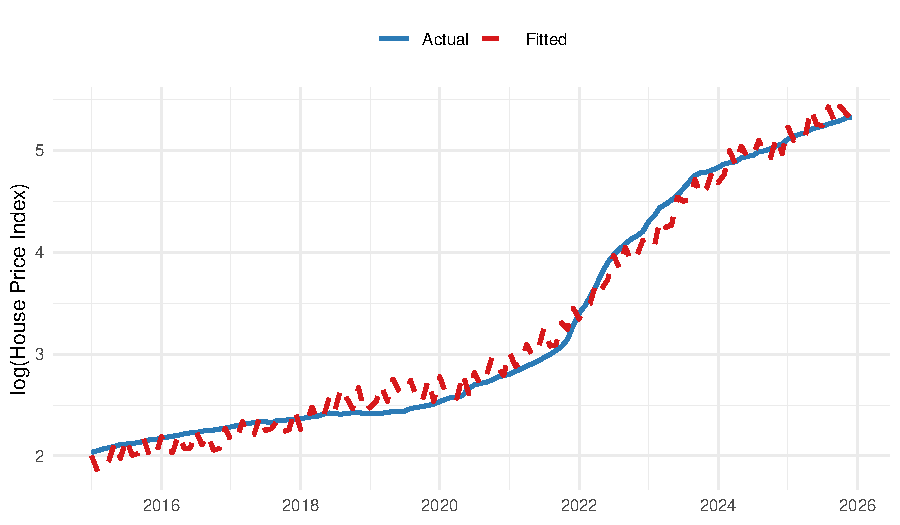
\includegraphics[keepaspectratio]{FAVURAL_EMU660_MiniPaper_files/figure-pdf/fig-fitted-1.pdf}}

}

\caption{\label{fig-fitted}Actual and fitted log(HPI) --- full model.}

\end{figure}%

The fitted values closely track the actual series
(Figure~\ref{fig-fitted}), including the sharp acceleration after 2021.
Larger residuals appear in 2022, the period of the most extreme TRY
depreciation, suggesting mild non-linearity at the most extreme
observations --- a limitation of the log-linear specification.

\subsubsection{Residual Plot}\label{residual-plot}

\begin{figure}[H]

\centering{

\pandocbounded{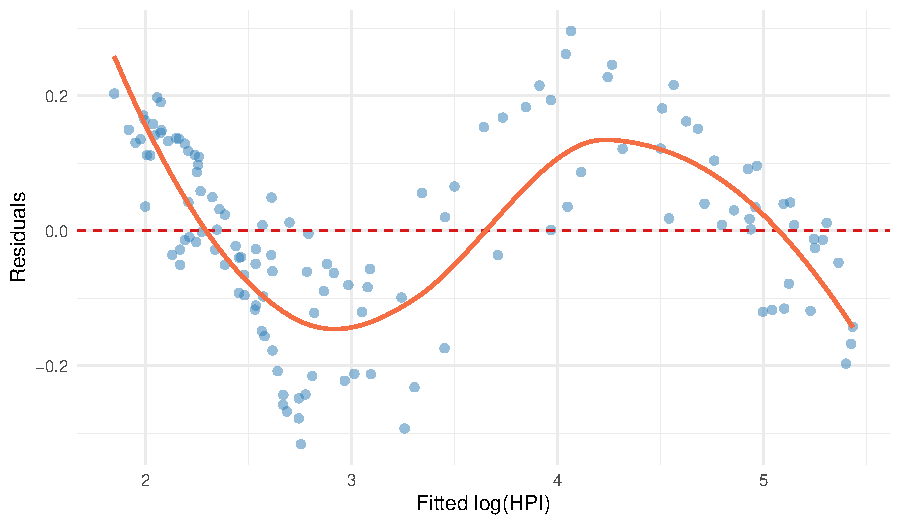
\includegraphics[keepaspectratio]{FAVURAL_EMU660_MiniPaper_files/figure-pdf/fig-residuals-1.pdf}}

}

\caption{\label{fig-residuals}Residuals vs.~fitted values --- full
model. The LOESS smoother (orange) reveals mild non-linearity at high
fitted values.}

\end{figure}%

Residuals are small and centred near zero for most of the fitted range
(Figure~\ref{fig-residuals}). Slight curvature at the upper end
corresponds to the 2022--2023 period of extreme depreciation and
confirms that a more flexible non-linear model could reduce this bias.

\section{Results and Key Takeaways}\label{sec-results}

The following conclusions emerge from the analysis:

\begin{enumerate}
\def\labelenumi{\arabic{enumi}.}
\item
  \textbf{House prices increased dramatically after 2020.} The national
  HPI shows a sharp acceleration during 2021--2023, more than doubling
  within a few years.
\item
  \textbf{Exchange rate depreciation is the strongest macroeconomic
  correlate.} USD/TRY and EUR/TRY each correlate with the HPI at
  \(r \approx 0.99\), and the baseline regression estimates an
  elasticity of approximately 1.20.
\item
  \textbf{Sales volume does not explain the price increase.} Housing
  sales are volatile and do not trend upward with the HPI, supporting
  the interpretation of affordability-driven demand compression at
  elevated price levels.
\item
  \textbf{Credit card expenditure reflects the general nominal inflation
  environment.} Its strong correlation with the HPI should be understood
  as evidence of economy-wide nominal expansion rather than direct
  housing demand.
\item
  \textbf{The price surge is nationwide but regionally uneven.} Coastal
  and western regions (Aegean, Marmara) experienced the strongest
  percentage growth; İstanbul leads in absolute terms. All regions,
  however, recorded extraordinary nominal appreciation.
\item
  \textbf{Results are statistically strong but should be interpreted
  cautiously.} All key variables are non-stationary and share a common
  nominal inflation trend. The analysis demonstrates strong association
  rather than definitive causality.
\item
  \textbf{Further research could improve causal identification.}
  Inflation-adjusted house prices, mortgage interest rates, housing
  credit volumes, construction cost indices, migration flows, and
  dynamic time-series methods (VAR, error-correction models) would
  strengthen the analysis.
\end{enumerate}

\section{Conclusion}\label{conclusion}

This study set out to explain why house prices in Türkiye have risen
sharply over the past decade. Drawing on official EVDS monthly
time-series data and applying exploratory analysis, correlation testing,
regional comparison, and multiple log-log regression, we find that
exchange rate depreciation and the broad nominal inflation environment
are the central drivers. A simple regression on the USD/TRY rate alone
explains nearly 96\% of the variation in the national HPI; adding sales
volume and credit card expenditure raises explained variance to
approximately 99\%.

These findings carry implications for policy. To the extent that housing
prices are driven by macroeconomic instability and currency depreciation
rather than local demand fundamentals, interventions targeted solely at
the housing market --- such as zoning changes or sales restrictions ---
are unlikely to be sufficient without broader macroeconomic
stabilisation.

The analysis has important limitations: it is conducted on nominal
series without stationarity corrections, and causal claims require
stronger identification assumptions than those employed here. Future
work should incorporate real prices, interest rates, and panel or
time-series cointegration methods to deepen the causal interpretation.

\newpage

\section*{References}\label{references}
\addcontentsline{toc}{section}{References}

Central Bank of the Republic of Türkiye (TCMB). (2024). \emph{Electronic
Data Delivery System (EVDS)}. Retrieved from
\url{https://evds2.tcmb.gov.tr/}




\end{document}
